\documentclass[a5paper]{article}

\usepackage{amsmath, amssymb}
\usepackage[margin=0.75in]{geometry}
\usepackage{graphicx}
\graphicspath{ {../../../Images/MATH11219/} }
\usepackage[hidelinks]{hyperref}
\usepackage{tikz}
\usepackage{stix}
\usepackage{pgfplots}
\pgfplotsset{compat=1.18}

\date{27\textsuperscript{th} of Jan 2026}
\setcounter{section}{0}

\begin{document}
	\begin{titlepage}
		\centering
		{\Huge \textsc{MATH11219}\par}
		\vspace{1cm}
		{\Large \textsc{Lecture Notes}\par}
		\vspace{2.5cm}
		\vfill
		Authored by\par
		Lachlan J. W. Wyer
		\vfill
		\makeatletter
		{\large Document Start Date: \@date \par}
		\makeatother
		{\large Latest Update: \today\par}
	\end{titlepage}
	\tableofcontents
	\pagebreak

	\section{Differentiation}
	Differentiation (Derivatives) is just a mathematical expression of a functions rate-of-change. Think of the gradient of a function, area/estimation of a function, kinematics \& optimisation of area or numbers.
	\subsection{Average Rate-of-Change (ARoC):}
	The ARoC of the function is just the estimation of a curve based on a linear lines gradient. I.E. the average gradient between two points.
	$$\text{ARoC}=\frac{y_{2}-y_{1}}{x_{2}-x_{1}}$$
	\subsection{Instaneous Rate-of-Change (IRoC):}
	The ARoC of a function is good enough to understand the general direction in which a graph is continuing. Its accuracy can be improved by limiting the amount of change between $x_{1}$ \& $x_{2}$. However a problem occurs when $\Delta x\rightarrow0$. As cannot divide by 0. To find a functions IRoC, use the derivatives by first principles.
	\begin{align*}
		f(x)&=3x^{2}+2\\
		f'(x)&=\lim_{\delta x \to 0}\frac{f(x+\delta x)-f(x)}{\delta x}\\
		     &=\lim_{\delta x \to 0}\frac{[3(x+\delta x)^{2}+2]-[3x^{2}+2]}{\delta x}\\
		     &=\lim_{\delta x \to 0}\frac{[3x^{2}+6x\delta x+3\delta x^{2}+2]-[3x^{2}+2]}{\delta x}\\
		     &=\lim_{\delta x \to 0}\frac{6x\delta x+3\delta x^{2}}{\delta x}\\
		     &=\lim_{\delta x \to 0}6x+3\delta x\\
		     &=6x
	\end{align*}
	\subsection{Limits in Functions:}
	Specifically in Piece-wise functions there can be an issue with derivatives and their interpretations. This is mostly around when the Left and Right Hand Limits not meeting on the same point, making the functions discontinuous.
	\pagebreak

	\begin{center}
		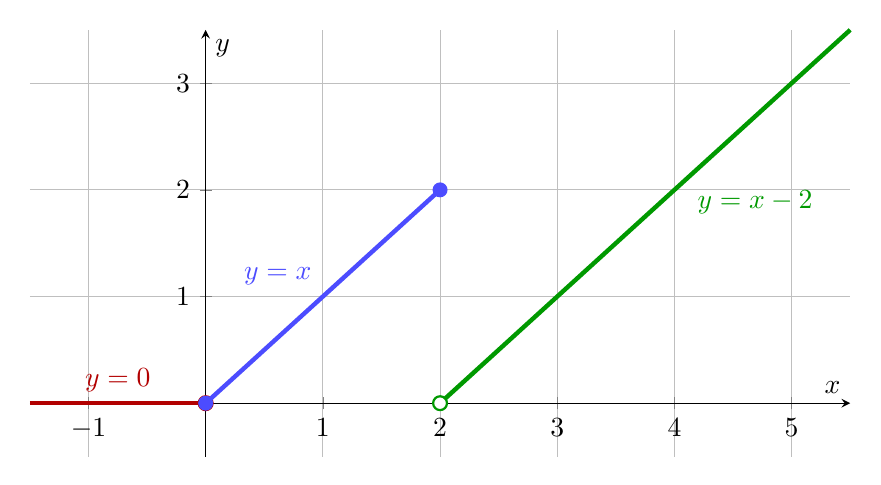
\begin{tikzpicture}
        \begin{axis}[
            axis lines = middle,
            xlabel = {$x$},
            ylabel = {$y$},
            grid = both,
            major grid style = {lightgray},
            minor grid style = {lightgray!25},
            width=12cm,
            height=7cm,
            xmin = -1.5, xmax = 5.5,
            ymin = -0.5, ymax = 3.5,
            xtick distance = 1,
            ytick distance = 1,
            % This helps position the labels (nodes) properly
            clip=false 
        ]

        % 1. Red Line: y = 0 {x < 0}
        \addplot[domain=-1.5:0, samples=2, color=red!70!black, ultra thick] {0}
            node[pos=0.5, above] {$y=0$};
        % Open circle at (0,0) for the red line
        \draw[red!70!black, thick, fill=white] (axis cs:0,0) circle (2.5pt);

        % 2. Blue Line: y = x {0 <= x <= 2}
        \addplot[domain=0:2, samples=2, color=blue!70!white, ultra thick] {x}
            node[pos=0.5, above left] {$y=x$};
        % Solid dots at (0,0) and (2,2)
        \addplot[only marks, mark=*, mark size=2.5pt, color=blue!70!white] coordinates {(0,0) (2,2)};

        % 3. Green Line: y = x - 2 {2 < x}
        \addplot[domain=2:5.5, samples=2, color=green!60!black, ultra thick] {x-2}
            node[pos=0.6, below right] {$y=x-2$};
        % Open circle at (2,0) for the green line
        \draw[green!60!black, thick, fill=white] (axis cs:2,0) circle (2.5pt);

        \end{axis}
    \end{tikzpicture}
	\end{center}
\end{document}
